\documentclass[12pt,a4paper,oneside]{article}
\usepackage{amssymb}
%0-\documentclass[a4paper,12pt]{article}
%\documentclass[prd,twocolumn]{revtex4}
%\documentclass[prd,a4paper]{revtex4}
\usepackage{epsfig}
%\usepackage[dvips]{graphicx}
\usepackage{graphicx}
\usepackage{multicol}
\usepackage{multirow}
%\usepackage[pdftex,bookmarksnumbered, pdfstartview=FitH,colorlinks,citecolor=blue,linkcolor=blue]{hyperref}
%\usepackage[dvipdfmx, bookmarksnumbered, pdfstartview=FitH,colorlinks,citecolor=blue,linkcolor=blue]{hyperref}
\usepackage[perpage,symbol]{footmisc}
\usepackage{subfigure}
\setfnsymbol{wiley}


%\Requirepackage{xspace}
%\tightenlines
\setlength{\oddsidemargin}{0.1cm} \setlength{\topmargin}{0.0cm}
\setlength{\textwidth}{17.0cm} \setlength{\textheight}{24.0cm}

\begin{document}
\newpage
Pic\\
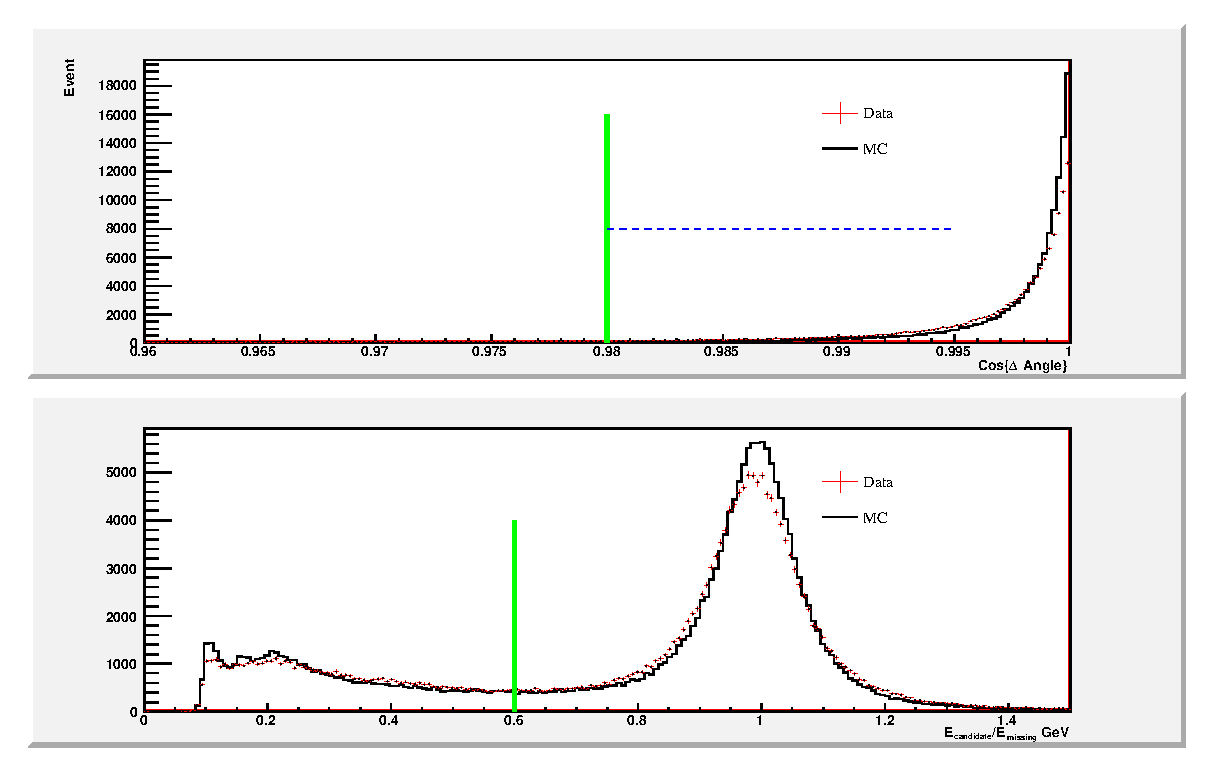
\includegraphics[width=2.2in,angle=0]{numerp_region.eps}
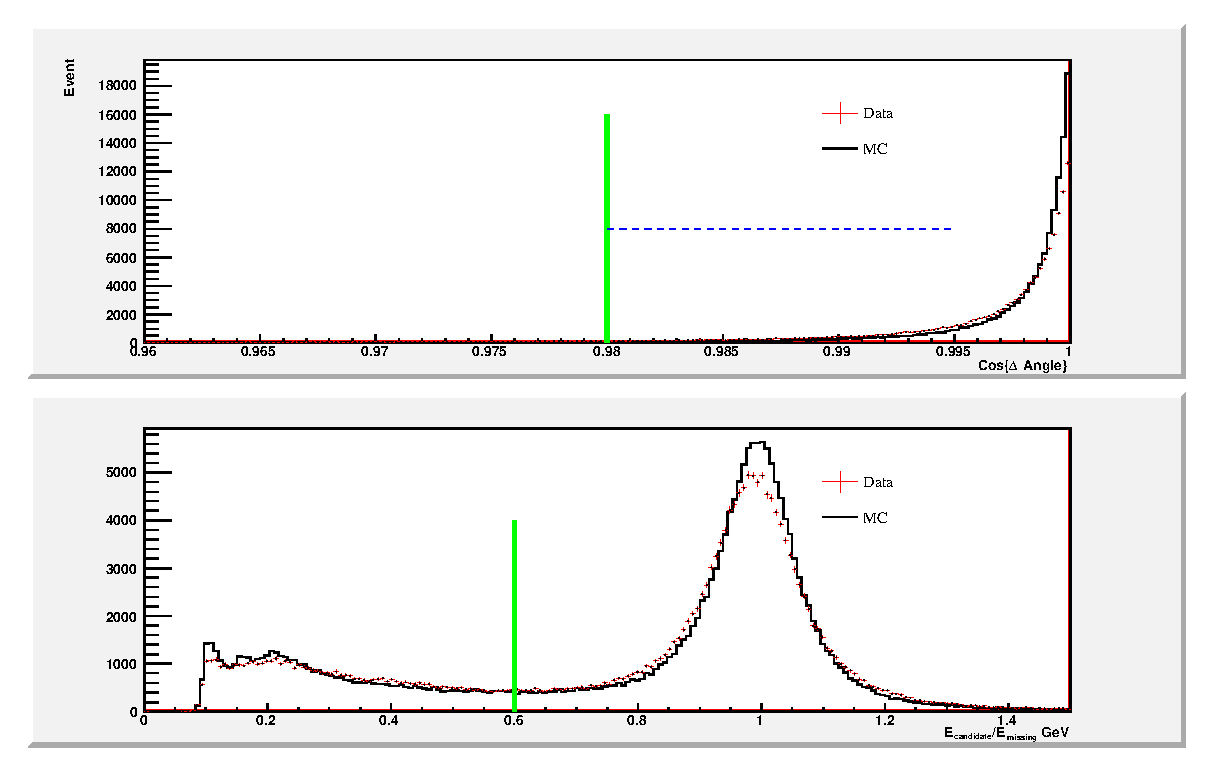
\includegraphics[width=2.2in,angle=0]{numerp_region.eps}\\
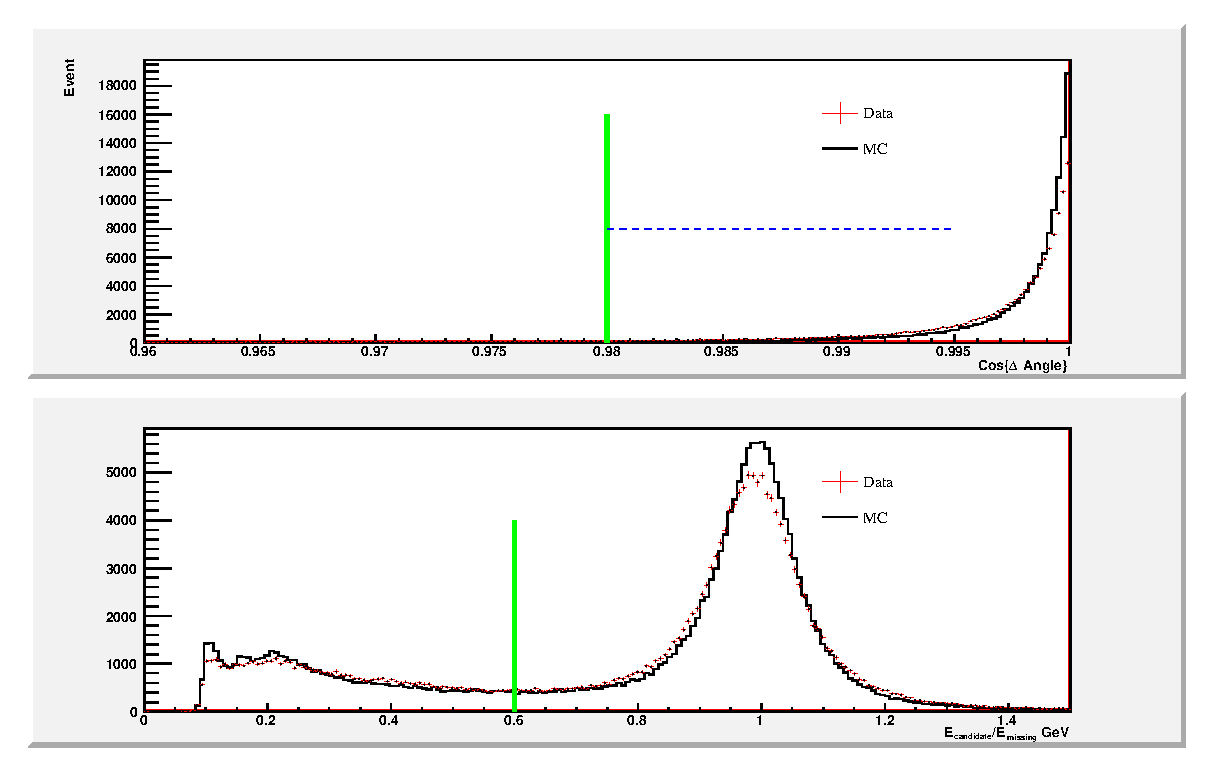
\includegraphics[width=2.2in,angle=0]{numerp_region.eps}
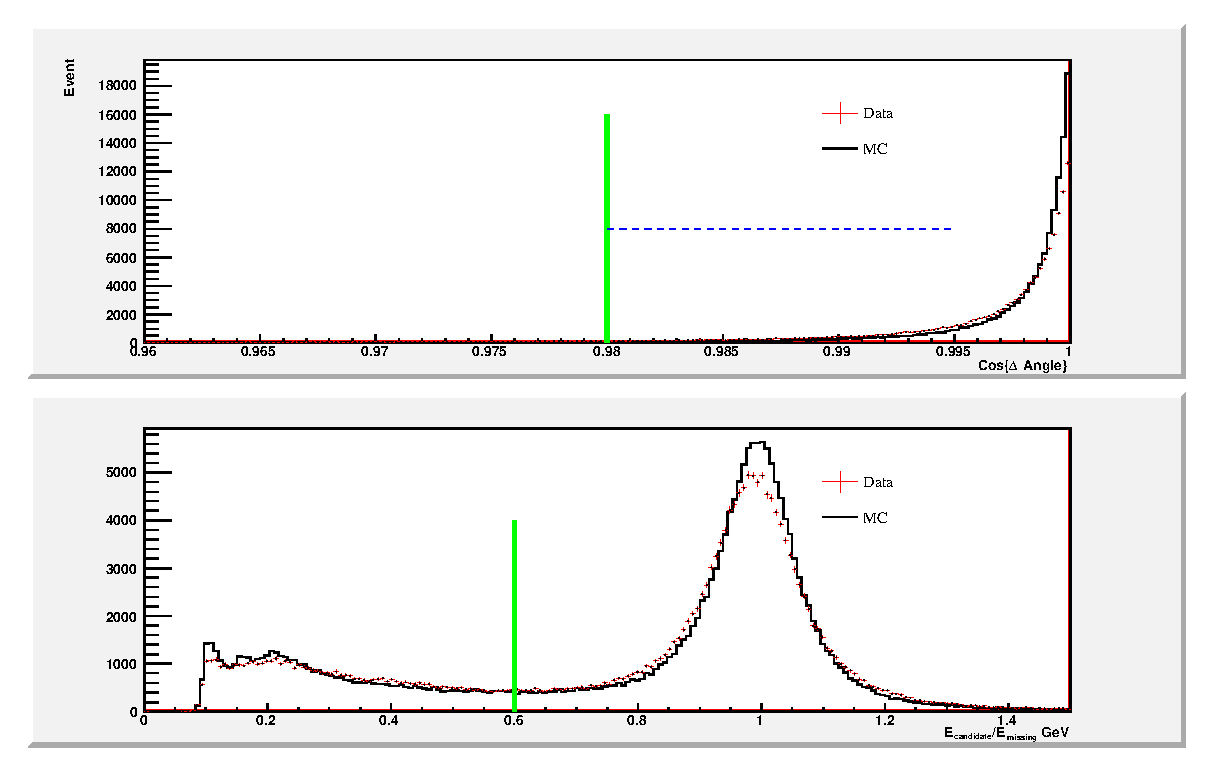
\includegraphics[width=2.2in,angle=0]{numerp_region.eps}\\
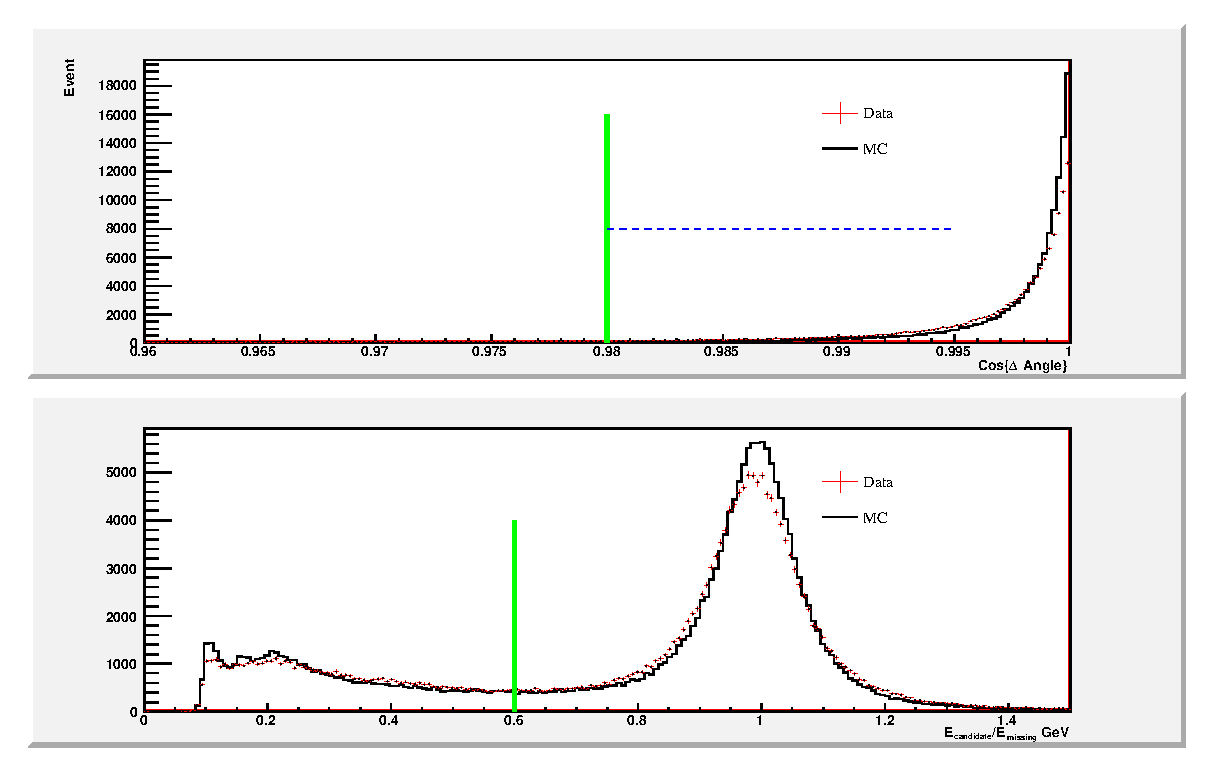
\includegraphics[width=2.2in,angle=0]{numerp_region.eps}
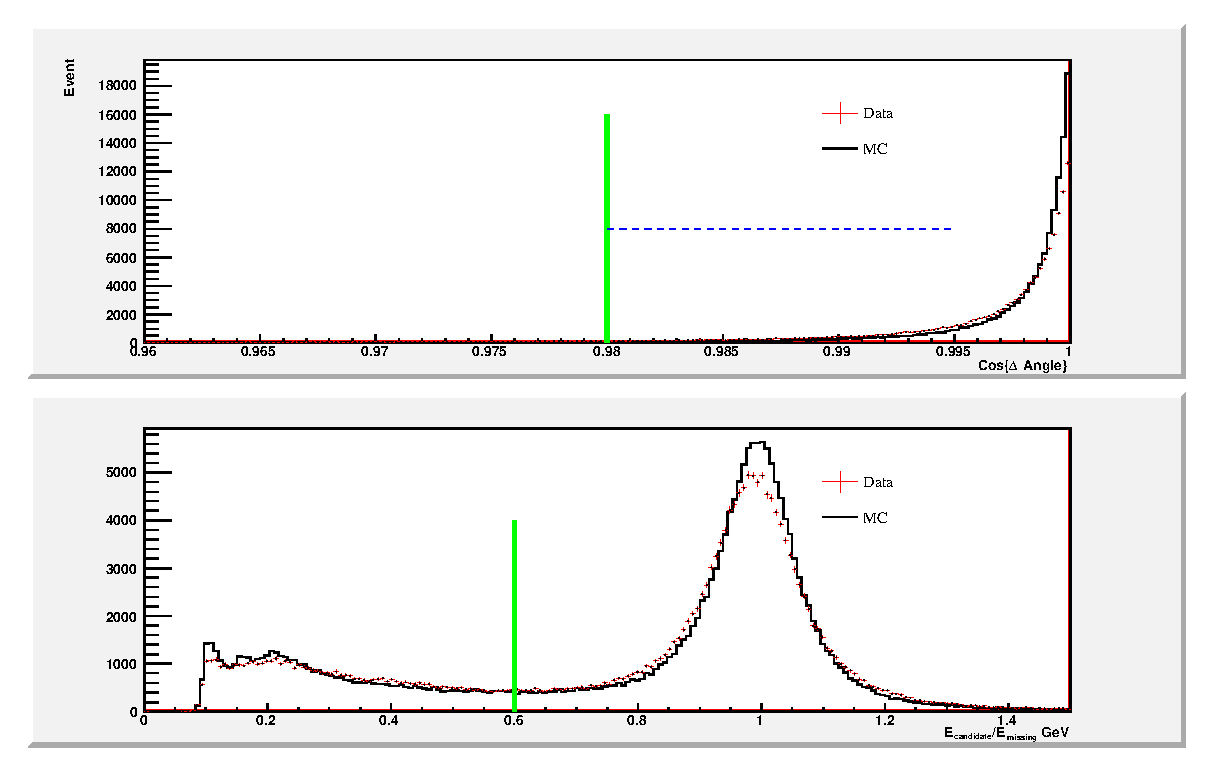
\includegraphics[width=2.2in,angle=0]{numerp_region.eps}\\
%
%\input{chap4/Eventsel.tex}
%
%\input{chap5/BGsuppression.tex}
%
%\newpage
%\input{chap6/psipp_gammaEtac.tex}
%\clearpage
%\input{chap7/psipp_gammaEtacp.tex}
%
%\newpage
%\input{chap8/SysError.tex}
%
%\input{chap9/Results.tex}
%
%\newpage
%\input{appendix.tex}
\end{document}

